\documentclass{beamer}
\usepackage[latin1]{inputenc}
\usepackage{graphicx}
\usepackage{longtable}
\usepackage{multicol}
\usepackage{biblatex}
\usepackage{tabularx}
\bibliography{gridbib}
\usetheme{Madrid}
\usebackgroundtemplate{
\setlength{\unitlength}{1mm}
\begin{picture}(-10,80)
%\put(5,-10){\includegraphics[scale=0.2]{Logo-v2.pdf}}
\put(95,-10){
\includegraphics[scale=0.1]{../logowork/doe-is-enes.pdf}}
\end{picture}
\setlength{\unitlength}{1pt}
}

\title{Scalable ESGF Node Manager}
\author{Sasha Ames / Prashanth D.}
\institute{LLNL / LIU}
\date{March 3 2015}
\begin{document}

\begin{frame}
\titlepage
\setlength{\unitlength}{1mm}
\begin{picture}(-10,-10)
%\put(40,-10){\includegraphics[scale=0.3]{Triolith3.jpg}}
\end{picture}
\setlength{\unitlength}{1pt}
\end{frame}

\begin{frame}{Contents}
\tableofcontents
\end{frame}

\section{Background}
\begin{frame}{Background}
The current ESGF Node Manager handles:
\begin{itemize}
\item Node membership and status
\item Capturing metrics
\item Sharing node information across federations: certs, endpoints etc
\item A mechanism to share common configuration files.
\end{itemize}
Drawbacks
\begin{itemize}
\item Limited scalability.
\item P2P file/data exchange could be more secure, particularly configuration files.
\end{itemize}

\end{frame}

\section{Desirable features for next-gen Node Manager}
\begin{frame}{Desirable features for next-gen Node Manager}
\begin{itemize}
\item Fault-tolerant distributed system, without a single point of failure
\item High scalability without overloading resources
\item Minimise communication overheads
\item PAN federation administration: handling cert requests, node memberships, etc.
\item Consistent and highly available common configuration files
\item Mechanism to enable component redundancy via consistency
\end{itemize}
\end{frame}

\section{Node Manager types}
\begin{frame}{Node Manager types}
Node managers can be of three different types.
\begin{enumerate}
\item Supernodes
\begin{itemize}
\item A validated and reliable source for configuration directives, metrics, information about components, etc., at project level.
\item Multiple concurrent supernodes for scalability, fault tolerance and load sharing.
\item Supernodes query other Node Managers for metrics and status.
\item A single Node Manager can serve as supernode to multiple projects or even as supernode to one and membernode to another etc.
\item Administrator action required to add/remove from ESGF
\end{itemize}
\item Membernodes
\begin{itemize}
\item Default Node Manager configuration
\item Cannot query other Node Managers.
\item May join or leave ESGF "at will"
\end{itemize}
\item Standby supernodes
\begin{itemize}
\item The Node Managers run as supernodes only when too few supernodes are operational.
\end{itemize}
\end{enumerate}
\end{frame}



\section{View of federated Node Managers}
\begin{frame}{View of federated Node Managers with projects }
\begin{center}
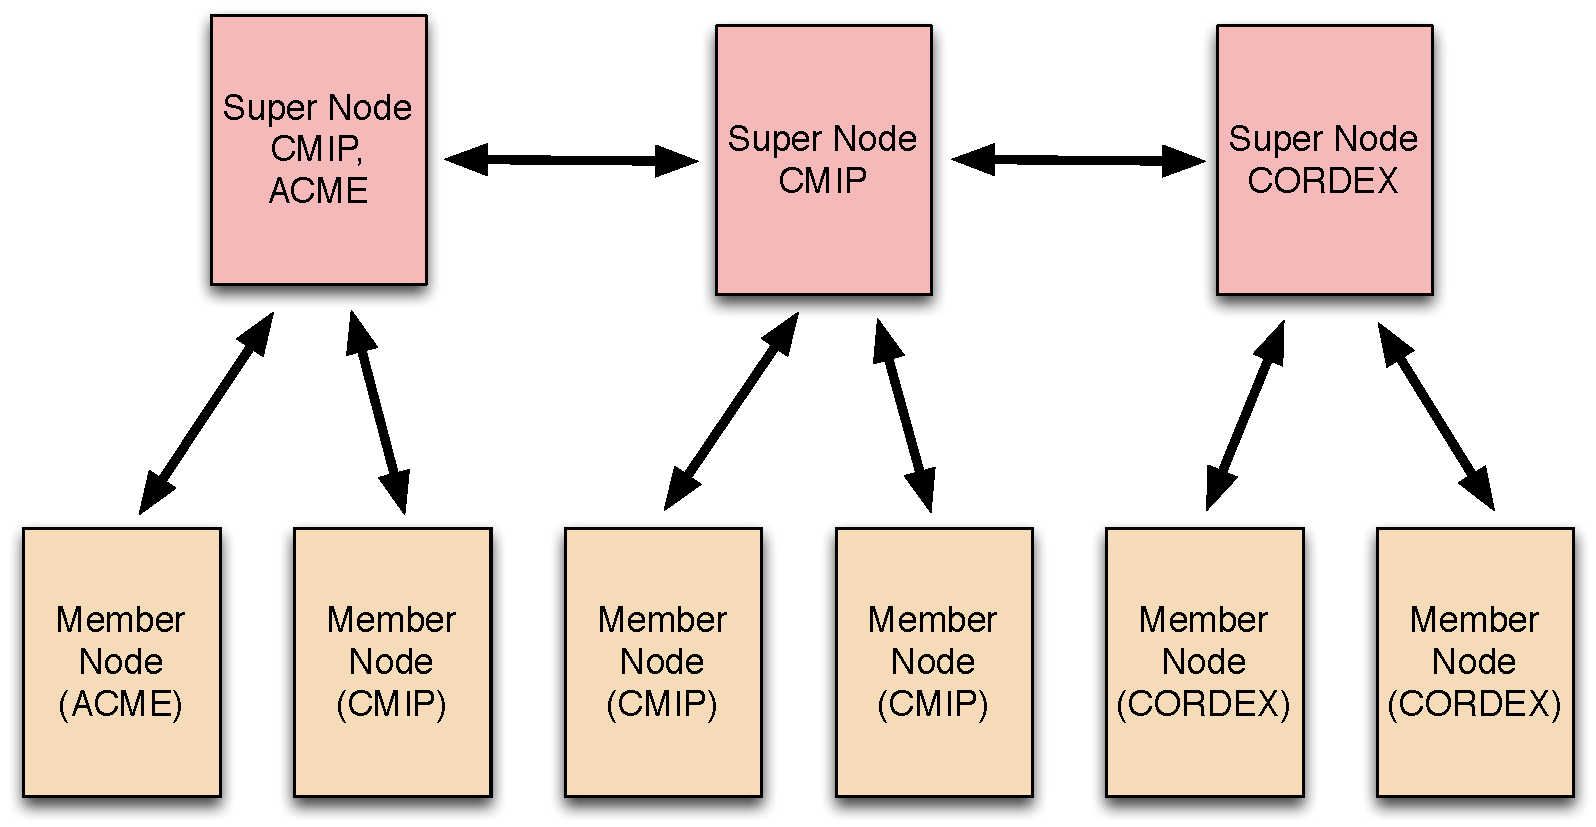
\includegraphics[scale=0.35]{ESG-node-org.pdf}
\end{center}
\end{frame}

\section{Node Manager role in ESGF Node}
\begin{frame}{Node Manager role in ESGF Node}

\begin{columns}
\begin{column}{.5\linewidth}

\tiny
\begin{tabularx}{6cm}{|c|X|}

\hline
Dashboard &  Manage consistent updates to registration.xml \\
\hline
Metrics & Coordinate metric metadata \\
\hline
Compute & Maintain repository of federated compute resources \\
\hline
Security & Replication of attributes for service failover \\
\hline
Update Manager & Consistent record of component versions \\
\hline
Notification & Push alert messages out to administrators / users \\
\hline
Replication & Data set version information \\
\hline
Publication & Consistent project-based configuration \\
\hline
Provenance & Consistent provenance metadata \\
\hline
Thredds & ??? \\
\hline
SOLR & ??? \\
\hline
CoG & ??? \\
\hline
Logger & (metadata)? \\
\hline
\end{tabularx}

\end{column}

\begin{column}{.5\linewidth}
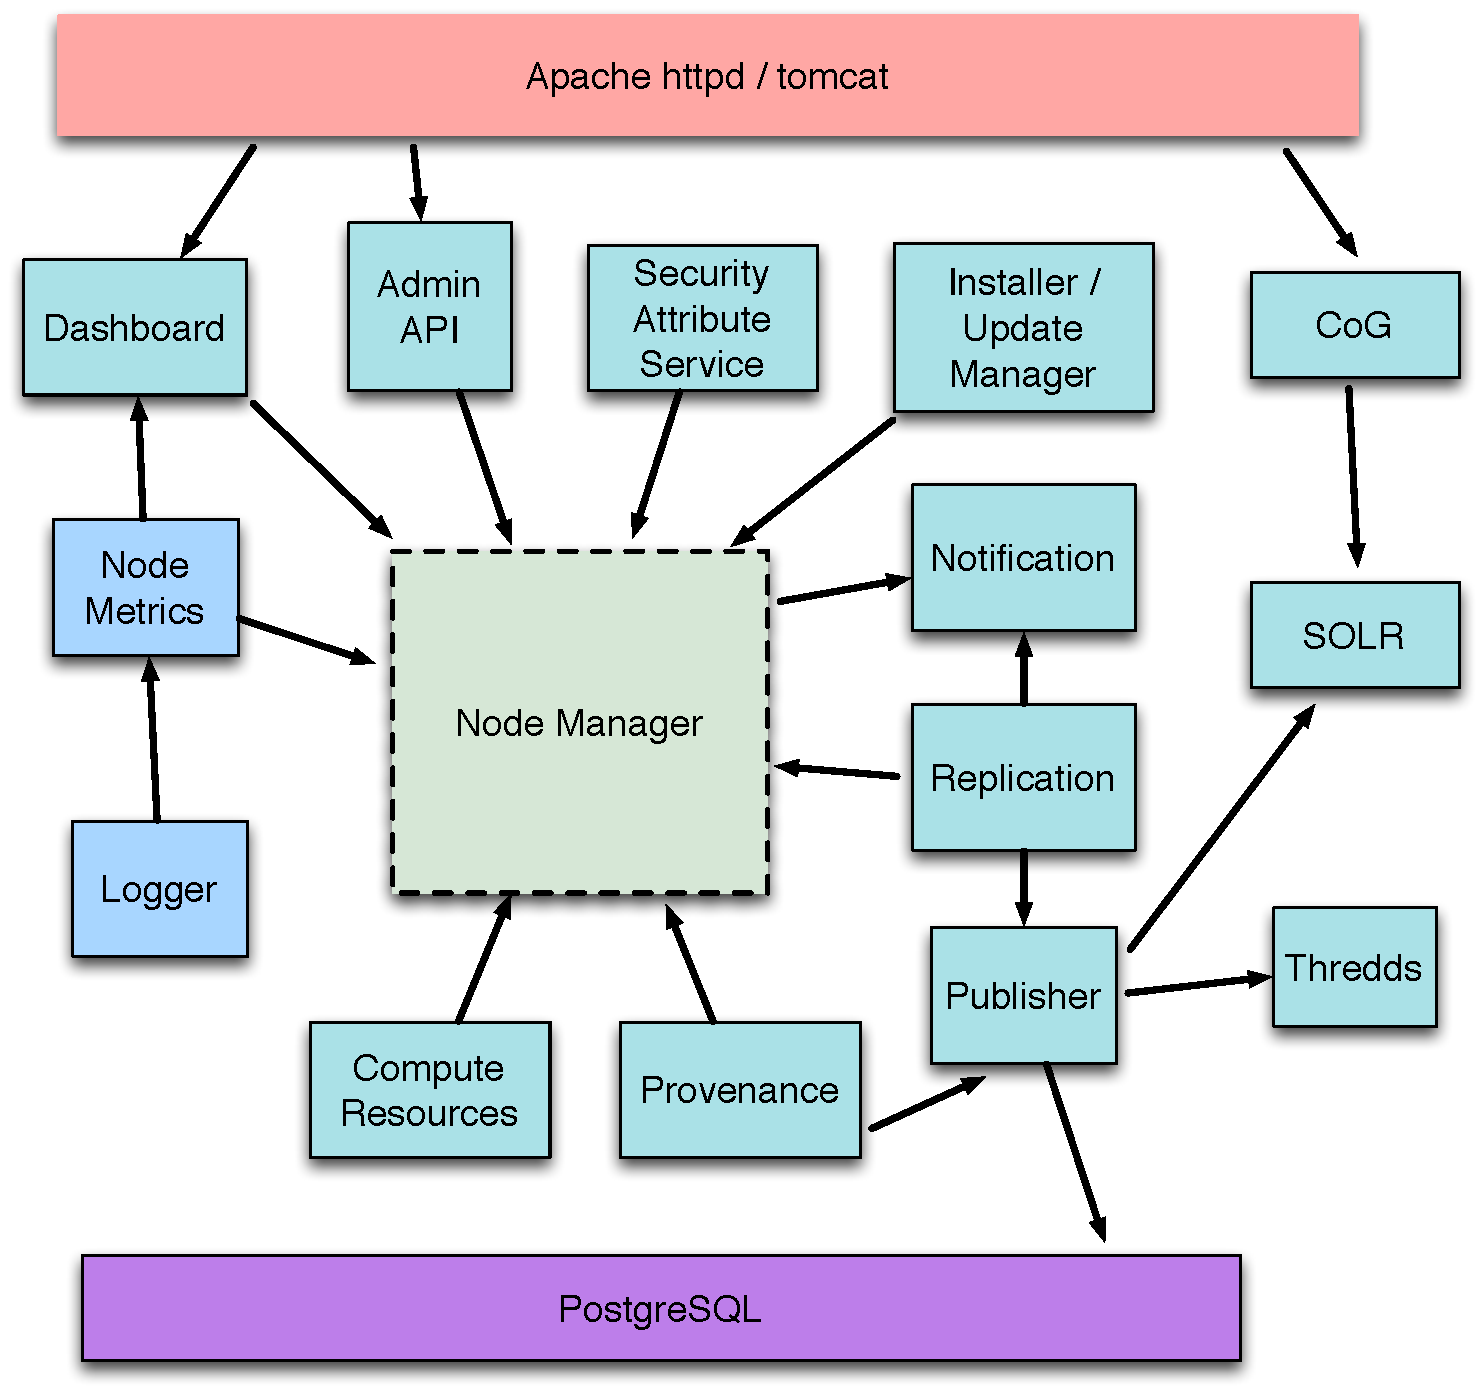
\includegraphics[width=\textwidth]{ESGF-node-components.pdf}
\end{column}
\end{columns}

\end{frame}

\section{Node Manager components}
\begin{frame}{Node Manager components}
\begin{itemize}

\item \textbf{Communication management}
\begin{itemize}
\item influenced by Zookeeper
\item Supernodes health check each other and member nodes
\item handles node failue
\end{itemize}


\item \textbf{ESGF Node Manager API} two subtypes
\begin{itemize}
\item P2P api - part of communication management
\item Services API - repository for ESGF components to share information, look up status
\end{itemize}


\item \textbf{Metric collector}: query member nodes and aggregate them (supernodes)
\item \textbf{Self-check component}: run sanity checks on self.



\item \textbf{Admin console (local node)}: submit membership requests, CSRs, volunteer for supernode role etc
\item \textbf{Admin console (supernode admin mode)}: sign CSRs, manage membership and volunteering requests etc. 
\end{itemize}
\end{frame}

%\Section{Services}
%
%\item \textbf{Messaging component}: alert notifications for local admins when services fail.
%
%
%Whem to Join 



\section{Node Manager component diagram}
\begin{frame}{Node Manager component diagram}
\begin{center}
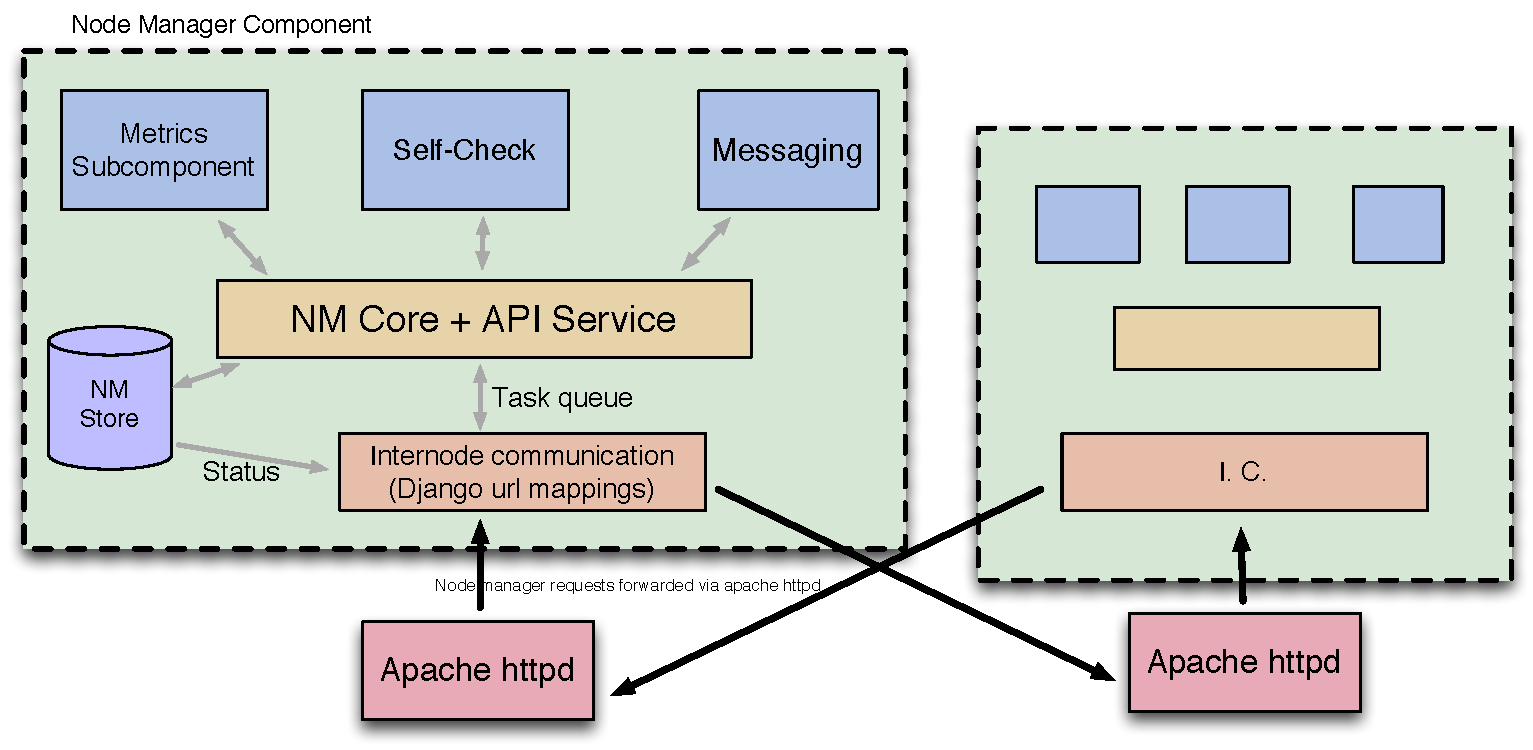
\includegraphics[scale=0.45]{NM-design-v2.pdf}
\end{center}
\end{frame}

\begin{frame}{Supernode failure mitigation}

\begin{itemize}
\item
Member nodes need to be redistributed for node-checks, file distribution in event the assigned supernode fails

\item
Option 1.  Distribute to active super nodes
\item
Option 2. Promote a standby node.  Distribute remaining nodes to "new" supernode, place of promoted node.
\item
Choice of options depends on setting, resources.  
\end{itemize}



\end{frame}

\begin{frame}{Supernode failure mitigation}

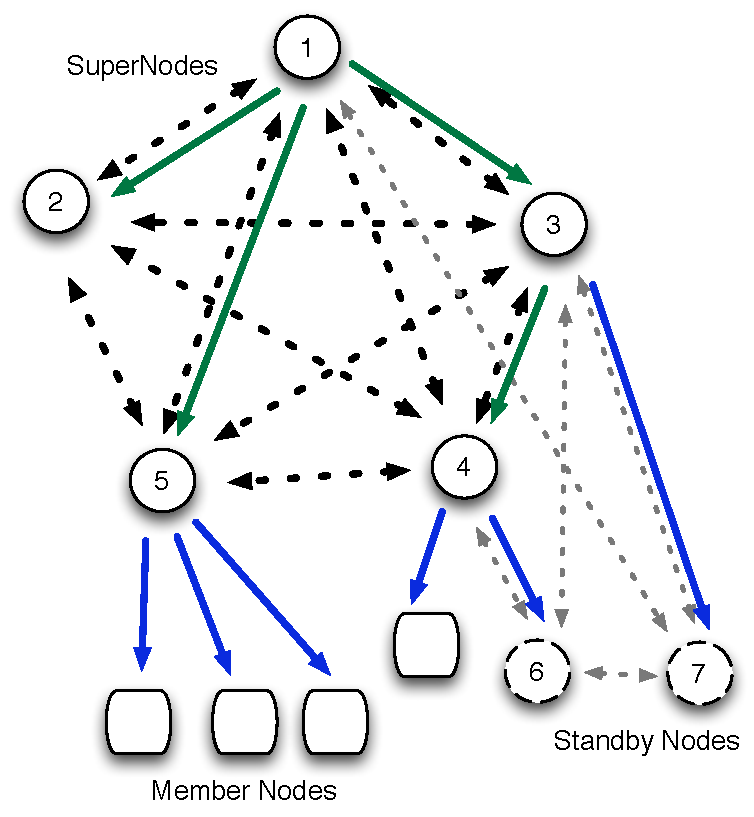
\includegraphics[scale=.5]{Node-comm-v3.pdf}


\end{frame}



\begin{frame}{Supernode failure mitigation}

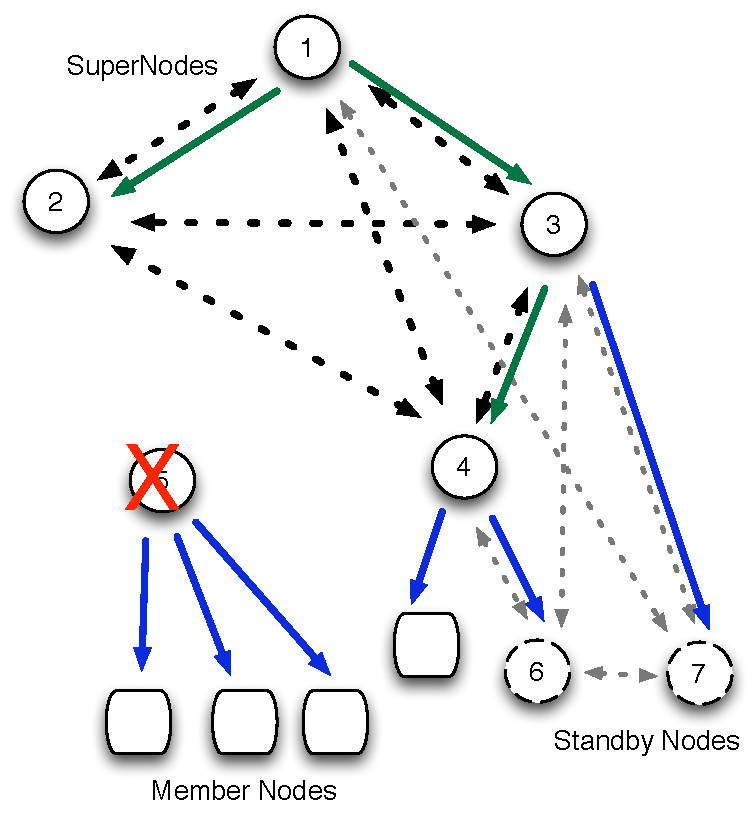
\includegraphics[scale=.5]{Node-comm-trans1.pdf}


\end{frame}

\begin{frame}{Supernode failure mitigation - Option 1}

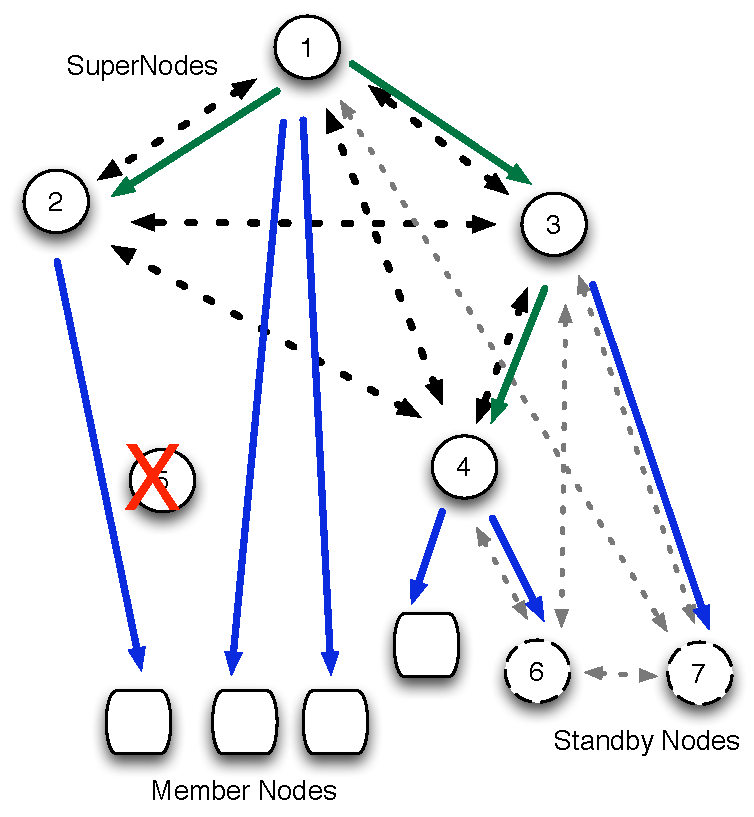
\includegraphics[scale=.5]{Node-comm-redist1.pdf}


\end{frame}


\begin{frame}{Supernode failure mitigation - Option 2}

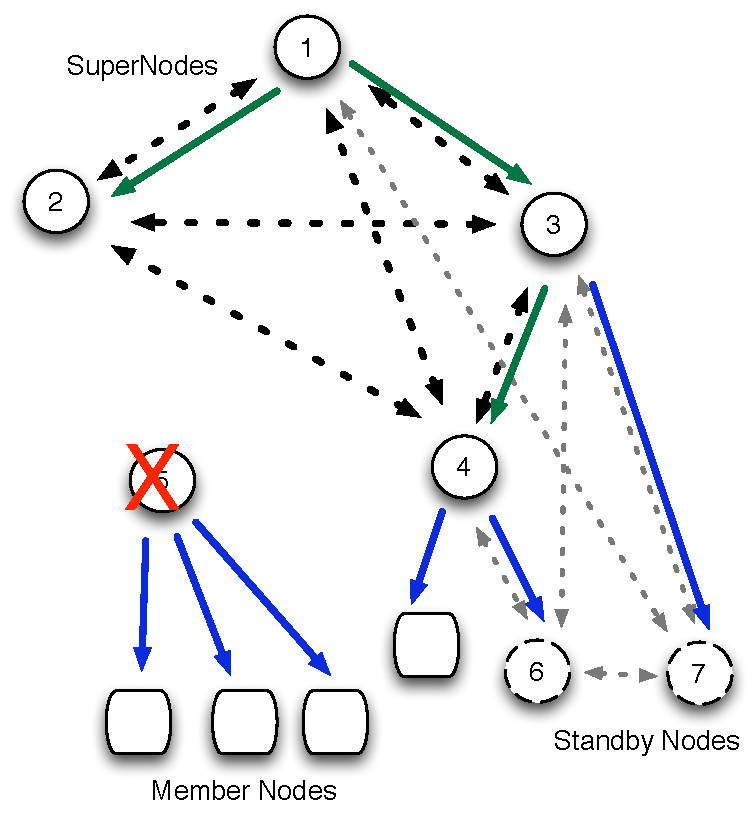
\includegraphics[scale=.5]{Node-comm-trans1.pdf}


\end{frame}


\begin{frame}{Supernode failure mitigation - Option 2}

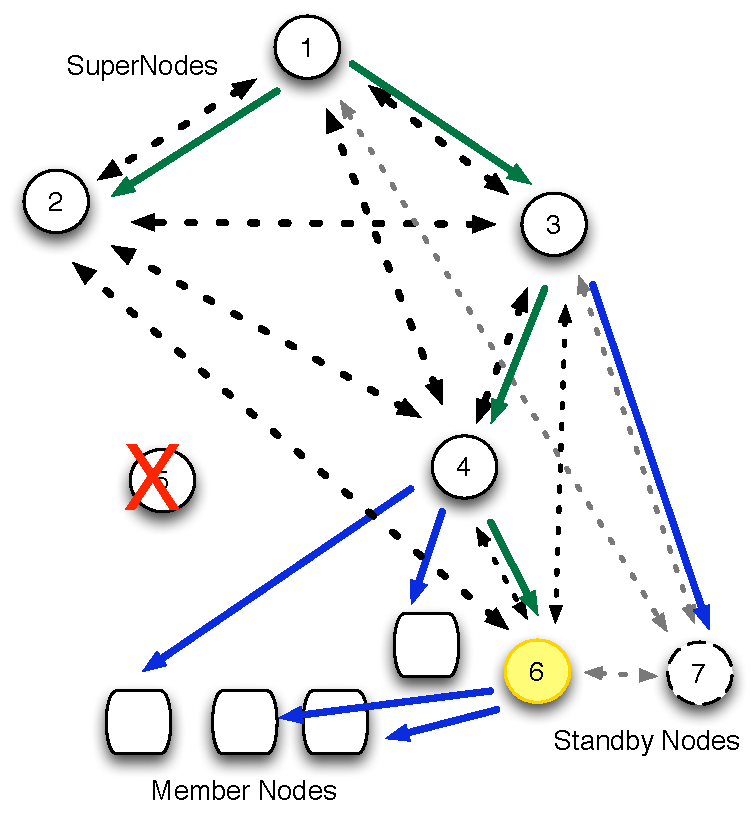
\includegraphics[scale=.5]{Node-comm-redist2.pdf}


\end{frame}


%\begin{columns}
%\begin{column}{.5\linewidth}
%
%\end{column}
%\begin{column}{.5\linewidth}
%
%\end{column}
%
%\end{columns}




\begin{frame}{Conflict resolution}
\begin{itemize}
\item
Modeled on git principles
\item
Changes are like commits with timestamps (supernode id becomes the "tiebreaker")
\item 
Deterministically ordered and replayed - all nodes get the same answer.
\item
Example: "race condition" of multiple member nodes joining in close succession. 

\end{itemize}



\end{frame}

\section{Prototyping}
\begin{frame}{Prototype of the Node Manager}
\begin{itemize}
\item
\textbf{API} Django
\begin{itemize}
 \item Supports node map distribution, member node join / self-removal.
\item
Passes work items (changes) to task queue
\end{itemize}
\item Task queue  - process changes.  Single worker handles updates synchronously

\item
Communication set up asynchronously. Responses added to queue.  

\end{itemize}

\end{frame}





\section{Future - Node Manager design considerations}
\begin{frame}{Node Manager design considerations}
\begin{itemize}
\item Security: factor for both user/machine executed elevated privilege operations.
\item Design to guard against spoofing of membernodes/supernodes etc.
\item 
Additional design and planning:
\item
\textbf{bootstrap:} how to stand up initial set of supernodes
\item
\textbf{transition roadmap} how to cut over from existing node manager without creating massive downtime for ESGF


\end{itemize}
\end{frame}

\section{Status of Effort}
\begin{frame}{Implementation Status}

\begin{itemize}
\item
Federation prototyping ongoing.   single source health check complete
\item
 Prototype implementation items to be completed
 \item
  node reassignment
\item
"multiple source" health check
\item

 conflict resolution
\item

 dashboard support
\item
Integrate django-based API with other django services running on ESGF node / httpd

 \item

Summer - start testing in wide-area environment - will need your help!
\end{itemize}
\end{frame}


\end{document}
